\documentclass{beamer}
\usetheme[hideothersubsections]{HRTheme}
\usepackage{beamerthemeHRTheme}
\usepackage{graphicx}
\usepackage[space]{grffile}
\usepackage{listings}
\lstset{language=SQL,
basicstyle=\ttfamily\footnotesize,
mathescape=true,
keywordstyle=\color{blue},
breaklines=true
showstringspaces=false}
\usepackage[utf8]{inputenc}
\usepackage{color}
\usepackage{wrapfig}
\newcommand{\red}[1]{
\textcolor{red}{#1}
}
\newcommand{\ts}{\textbackslash}
\newcommand{\valseq}[1]{$\lbrace$ #1 $\rbrace$}
\newcommand{\tuple}[2]{$t_{#1}$[#2]}
\newcommand{\fdep}[2]{#1 $\rightarrow$ #2}

\title{Introduction to normalization}

\author{TEAM INFDEV}

\institute{Hogeschool Rotterdam \\ 
	Rotterdam, Netherlands}

\date{}

\begin{document}
\maketitle

\SlideSection{Lesson overview}

\begin{frame}
	\frametitle{Lesson topics}
	\begin{itemize}
		\item Problems caused by bad database implementations.
		\item Reasons behind Normalization.
		\item Functional dependencies.
		\item Normal forms.
	\end{itemize}
\end{frame}

\SlideSection{Introduction}

\begin{frame}
	\frametitle{Introduction}
	\framesubtitle{Reasons behind normalization}
	\begin{itemize}
		\item It is a process to improve the design of the database.
		\item Objective 1: minimize the storage space used by the relations.
		\item Objective 2: eliminate anomalies in the database.
		\item Objective 3: eliminate spurious tuples.
	\end{itemize}
\end{frame}

\begin{frame}
	\frametitle{Introduction}
	Create tables with a lot of information is prone to waste of storage space.

	\begin{figure}
		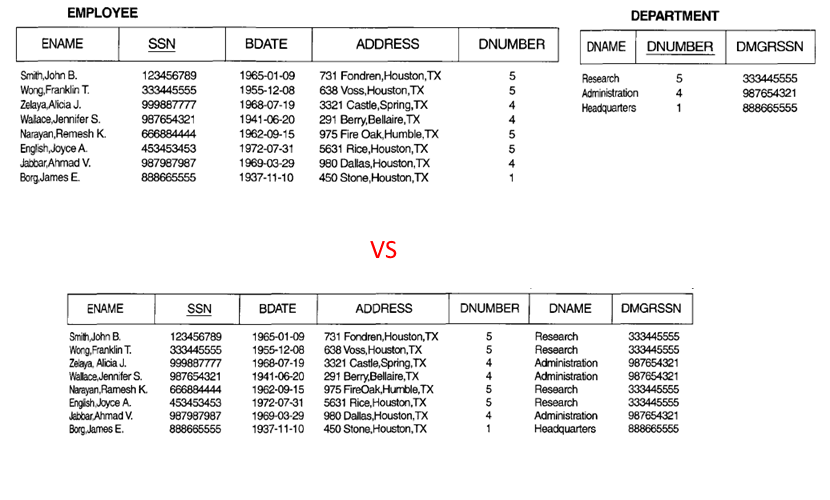
\includegraphics[scale=0.4]{img/normalization/norm1}
	\end{figure}
\end{frame}

\begin{frame}
	\frametitle{Introduction}
	\framesubtitle{Waste of storage space}
	\begin{itemize}
		\item Using two separate tables and joining them uses less storage space then putting everything in the same table.
		\item The values of the attributes of the department are repeated for every employee who works in that department.
		\item It means that, if a department has 300 employees, we waste 300 times the memory space than the approach with two tables.
	\end{itemize}
\end{frame}

\begin{frame}
	\frametitle{Introduction}
	\framesubtitle{Update Anomalies}
	\begin{figure}
		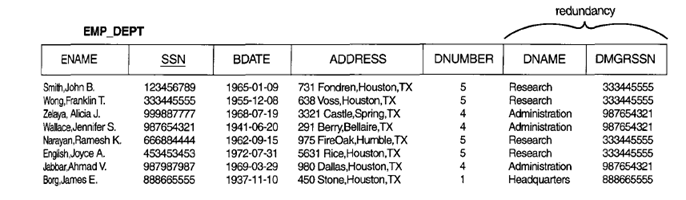
\includegraphics[scale = 0.45]{img/normalization/norm2}
	\end{figure}
	\begin{itemize}
		\item The values contained in \texttt{DNAME} are always coupled with the same values in \texttt{DMGRSSN}. For example ‘Research’ is always coupled with 333445555. This is called redundancy.
		\item Inserting a new employee requires to repeat this coupling manually (manual consistency).
		\item If you add a new department, then we have to enter a null value for each attribute of the employee.
	\end{itemize}
\end{frame}

\begin{frame}
	\frametitle{Introduction}
	\framesubtitle{Update Anomalies (deletion)}
	
	\begin{itemize}
		\item Deleting the tuple of the last employee of the department also removes all the information about that department.
		\item We must manually apply null values to the attributes of the employee in order to remove the last employee from the department.
		\item Example: Deleting Borg, James E. also removes all the information about the ‘Headquarters’ department.		
	\end{itemize}
\end{frame}

\begin{frame}
	\frametitle{Introduction}
	\framesubtitle{Update Anomalies (modification)}
	
	\begin{itemize}
		\item Modifying the information of a department in one tuple is not reflected in the other tuples.
		\item If we want to update the information about a department we must repeat the update for all the tuples containing the employees of that department	
		\item \textbf{Example:}  If we change the name of the department ‘Research’ into ‘Research and development’ we have to repeat this change for 4 tuples.			
	\end{itemize}
\end{frame}

\begin{frame}
	\frametitle{Introduction}
	\framesubtitle{Spurious tuples}
	
	\begin{figure}
		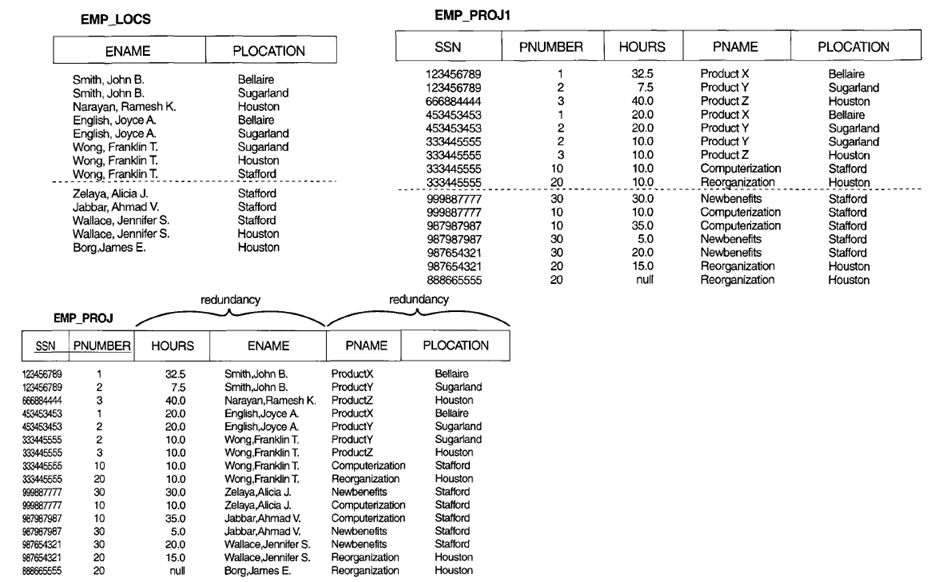
\includegraphics[scale=0.4]{img/normalization/norm3}
	\end{figure}
\end{frame}

\begin{frame}
	\frametitle{Introduction}
	\framesubtitle{Spurious tuples}
	
	\begin{itemize}
		\item Normalization uses decomposition to eliminate anomalies and remove redundancy.
		\item The two tables above in the previous slide are a decomposition of the bottom one.
		\item If we join the two tables, we get more tuples than those that were in the original table
		\item Those below the dotted line are extra tuples called spurious tuples.
		\item Normalization must ensure that the decomposition does not create spurious tuples after a join.
	\end{itemize}
\end{frame}

\begin{frame}
	\frametitle{Normal forms}
	\begin{itemize}
		\item Normalization is the process of converting the relations (tables) of a database into other relations in some normal form.
		\item Normal forms are properties that a relation must satisfy.
		\item There are two different kinds of definitions of normal forms:
		\item Historical definitions: The original definitions defined by Codd, taking into account only the primary key.
		\item Refined definitions: A refinement of the normal forms that takes into account also the candidate keys.		
	\end{itemize}
\end{frame}

\SlideSection{Normal forms}
\begin{frame}
	\frametitle{Normal forms}
	\framesubtitle{Functional dependencies}
	
	\begin{figure}
		
\includegraphics[scale=0.75]{img/normalization/mathiscoming}
	\end{figure}
\end{frame}

\begin{frame}
	\frametitle{Normal forms}
	\framesubtitle{Functional dependencies}
	\begin{itemize}
		\item Both kinds of definitions of normal forms rely on the concept of functional dependency.
		\item In what follows we write \tuple{i}{X} to indicate the values of the row i of a table for a set of attributes X
		\item \textbf{Example}: \tuple{3}{SSN,HOURS,NAME} in the table below is the combination of values: 
		\tuple{3}{SSN,HOURS,NAME} = \valseq{666884444,40.0,Narayan, Ramesh K.}
	\end{itemize}
	
	\begin{figure}
		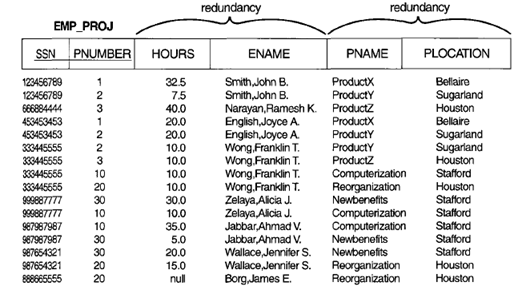
\includegraphics[scale=0.4]{img/normalization/norm5}
	\end{figure}
\end{frame}



\begin{frame}
	\frametitle{Normal forms}
	\framesubtitle{Functional dependencies}
	\textbf{Definition:}\\
	Given a subset of attributes X and Y in a relation, we say that Y depends on X, and we write \fdep{X}{Y}, if for any pair of rows where we have \tuple{i}{X} = \tuple{j}{X} we also have \tuple{i}{Y} = \tuple{j}{Y}.
	
	\tiny
	\textbf{Example: } In the table below we have, if we assume that there is a dependency \fdep{PNAME}{PLOCATION}, then when \tuple{i}{PNAME} = \tuple{j}{PNAME} we also have \tuple{i}{PLOCATION} = \tuple{j}{PLOCATION}. For instance every time we have the value 'ProductY' in the column PNAME, we also have 'Sugarland' in the column PLOCATION. It is not possible that a row has 'ProductY' in the column PNAME and 'Belaire' in the column PLOCATION.
	
	\begin{figure}
		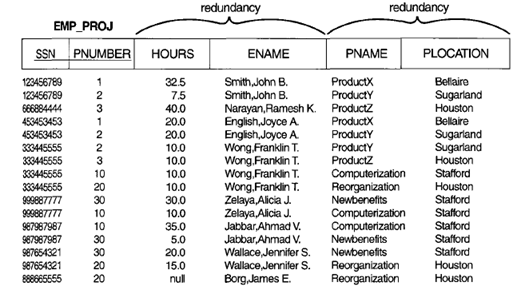
\includegraphics[scale=0.4]{img/normalization/norm6}
	\end{figure}
\end{frame}

\begin{frame}
	\frametitle{Functional dependencies}
	\framesubtitle{Important observations}
	
	\begin{itemize}
		\item Functional dependencies are defined by the database designer.
		\item It is not possible to infer functional dependencies by reading the data from the table.
		\item Functional dependencies should be read in the documentation of the database or asked to the designer.
		\item If you need to normalize a database and there is no documentation or the designer is unavailable, \textbf{\underline{as last resort}}, you can try to infer functional dependencies from the data.		
	\end{itemize}
\end{frame}

\begin{frame}
	\frametitle{Functional dependencies}
	\framesubtitle{Bad practice - An example}
	
	\begin{table}
		\begin{tabular}{|c|c|c|}
			\hline
			\underline{ssn} & name & salary\\
			\hline
			299260 & John Smith & 2500 \\
			\hline
			993693 & Walter White & 3000 \\
			\hline
			388528 & John Smith & 2500\\
			\hline
			396926 & James Garnett & 1800 \\
			\hline
		\end{tabular}
	\end{table}
	
	\pause
	By looking at the data in the table I could infer that \fdep{name}{salary} because two employees with the name John Smith earn 2500 euros per month.
	If later I add the tuple (395935,John Smith,2000) (another employee with the same name but different salary) the dependency is gone!
	This because clearly the salary of an employee should not depend on a person’s name, but this is what we could infer just by looking at the data.
	
\end{frame}

\begin{frame}
	\frametitle{Normal forms}
	\framesubtitle{1st Normal form}
	
	\begin{itemize}
		\item The first normal form is automatically granted by the relational model.
		\item If you designed the conceptual model properly and translated correctly the ERD into the relational model, then all your relations should be in 1NF.
	\end{itemize}
	
	\begin{wrapfigure}{r}{0.5\textwidth}
		%\vspace{-20pt}
		\begin{center}
			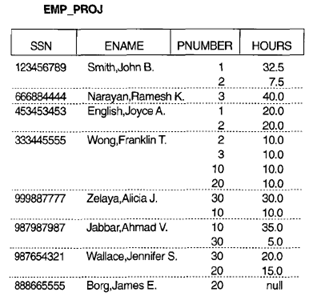
\includegraphics[scale=0.4]{img/normalization/norm7}
		\end{center}
		%\vspace{-20pt}
		%\vspace{-10pt}
	\end{wrapfigure}
	
	\textbf{Definition:}
	A table is in 1st normal form (1NF) if no row has multiple values for an attribute.
	
	\textbf{Example:} The table to the right violates the 1NF since some rows have multiple values for PNUMBER and HOURS.
\end{frame}

\begin{frame}
	\frametitle{Normal forms}
	\framesubtitle{2nd Normal form}
	
	\textbf{Definition:}
	A table is in 2nd normal form (2NF) if it is in 1NF and every attribute that is not part of a key depends on the whole primary key.
	
	\begin{wrapfigure}{r}{0.5\textwidth}
		%\vspace{-20pt}
		\begin{center}
			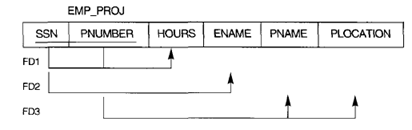
\includegraphics[scale=0.5]{img/normalization/norm8}
		\end{center}
		%\vspace{-20pt}
		%\vspace{-10pt}
	\end{wrapfigure}
	
	\textbf{Example:}
	The table to the right is not in 2NF because PNAME depends only on PNUMBER and not on the whole key. The same for PLOCATION
	
\end{frame}

\begin{frame}
	\frametitle{Normal forms}
	\framesubtitle{2nd Normal Form}
	
	\textbf{Useful trick:}
	If you have a table where the primary key is made of only one attribute, the table is always in 2NF. You can say this without any additional check
	
	\textbf{Why?}
	\pause
	Because to break the 2NF there must exist a functional dependency where the left side is a part of the primary key, but this is impossible if you have only one attribute.
\end{frame}

\begin{frame}
	\frametitle{Normal forms}
	\framesubtitle{2nd Normal Form - Reason}
	
	\begin{figure}
		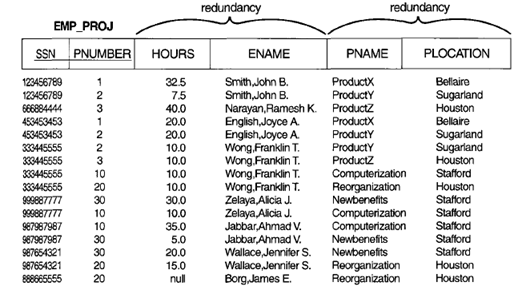
\includegraphics[scale=0.4]{img/normalization/norm10}
	\end{figure}
	
	If I want to assign an employee to an existing project, I have to manually repeat the data in PNAME and PLOCATION for the new tuple even if they already exist in other tuples.
	
	
	For example if I add the employee 394394343 to project 1, I have to repeat the values ProductX and Bellaire in the new tuple manually.
\end{frame}

\begin{frame}
	\frametitle{Normal forms}
	\framesubtitle{Transitive dependency}
	
	The 3rd normal form requires to define a \textit{transitive dependency}
	
	\textbf{Definition}:
	A functional dependency \fdep{X}{Y} is transitive if there is a set of attributes Z, which is neither a candidate key nor a subset of any key, and both \fdep{X}{Z} and \fdep{Z}{Y} are valid functional dependency
	
	\begin{figure}
		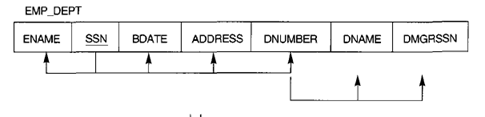
\includegraphics[scale=0.4]{img/normalization/norm9}
	\end{figure}
	
	\textbf{Example:}
	In the table above the functional dependency \fdep{SSN}{\valseq{DNAME,DMGRSSN}} is transitive because also \fdep{SSN}{DNUMBER} and \fdep{DNUMBER}{\valseq{DNAME,DMGRSSN}} are valid functional dependencies.	
\end{frame}

\begin{frame}
	\frametitle{Normal forms}
	\framesubtitle{Decomposition rule}
	
	\textbf{Another useful trick:}
	We do not give the proof of this, but remember that you can always decompose a functional dependency, with a right side containing more than one attribute, into two smaller functional dependencies. This procedure is recursive, so you can apply it again to the two functional dependencies created at the previous step.
	
	\textbf{Example:}
	\small
	\fdep{DNUMBER}{\valseq{DNAME,DMGRSSN}} can be decomposed into the two functional dependencies \fdep{DNUMBER}{DNAME} and \fdep{DNUMBER}{DMGRSSN}
	
\end{frame}

\begin{frame}
	\frametitle{Normal forms}
	\framesubtitle{3rd normal form}
	
	\textbf{Definition (3NF):}
	A table is in 3rd normal form (3NF) if it is in 2NF and no attribute that is not part of a key is transitively dependent on the primary key.
	
	\textbf{Example:}
	The table below is in 2NF but not in 3NF because of the transitive dependency \fdep{SSN}{\valseq{DNAME,DMGRSSN}}
	\begin{figure}
		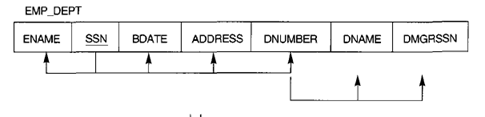
\includegraphics[scale=0.4]{img/normalization/norm9}
	\end{figure}
\end{frame}

\begin{frame}
	\frametitle{Normal forms}
	\framesubtitle{3rd normal form - Reason}
	
	\begin{figure}
		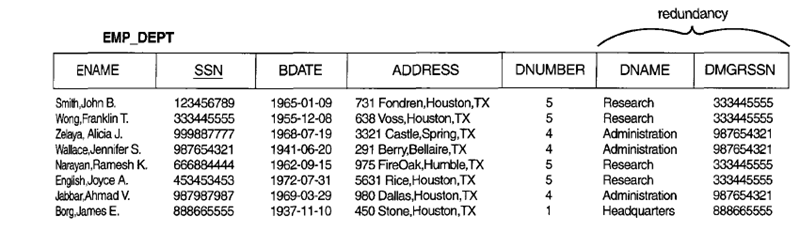
\includegraphics[scale=0.4]{img/normalization/norm11}
	\end{figure}
	
	If I add a new employee to a department I have to repeat DNAME and DMGRSSN for that department because of the transitive dependency.
	
	If I add employee 394394343 to department number 5 I have to repeat the value Research and 333445555 for that department manually.	
\end{frame}

\SlideSection{General normal forms}

\begin{frame}
	\frametitle{Normalization on candidate keys}
	
	\begin{itemize}
		\item All the normal forms defined so far are defined for the primary key only.
		\item Anomalies might aries also with depndencies on the candidate key.
		\item We give more general definitions of normal forms that take into account also the candidate keys.
		\item The definition of 1NF is not affected since it only requires that each tuple has a single value for all the attributes (not based on a property on the primary key).		
	\end{itemize}
\end{frame}

\begin{frame}
	\frametitle{Normalization on candidate keys}
	\framesubtitle{General 2nd normal form}
	
	\textbf{Definition:}
	A table is in 2NF if every attribute that is not part of a key is not partially dependent on any key of the table (primary or candidate)
	
	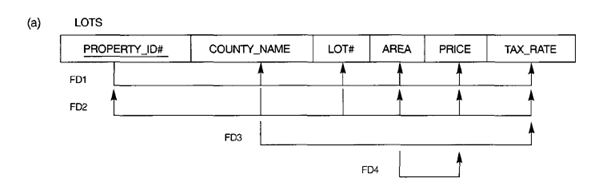
\includegraphics[scale=0.4]{img/normalization/norm12}
\pause	
	\textbf{Example:}
	The table is not in 2NF because a candidate key is
	
	\valseq{COUNTY\textunderscore NAME,LOT\#} 
	
	and the attribute TAX\textunderscore RATE depends on COUNTY\textunderscore NAME.
\end{frame}

\begin{frame}
	\frametitle{Normalization on candidate keys}
	\framesubtitle{General 2nd normal form - Reason}
	
	\begin{figure}
		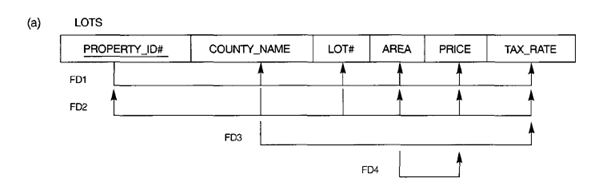
\includegraphics[scale=0.4]{img/normalization/norm12}
	\end{figure}
	
\pause
	If I want to add a new property in an existing COUNTY \textunderscore NAME, I have to manually repeat the data about TAX\textunderscore RATE.
\end{frame}

\begin{frame}
	\frametitle{Normalization on candidate keys}
	\framesubtitle{General 3rd normal form}
	
	\textbf{Trivial functional dependency:}
	A functional dependency 
	
	\fdep{X}{Y} 
	
	is trivial if Y is part of X.
	
	\textbf{Definition:}
	A table is in 3rd normal form if it is in 2NF and for any non-trivial functional dependency \fdep{X}{A} one of the two conditions is satisfied:
	\begin{enumerate}
		\item X is a superkey.
		\item A is part of a key.
	\end{enumerate}
\end{frame}

\begin{frame}
	\frametitle{Normalization on candidate keys}
	\framesubtitle{General 3rd normal form - Reason}
	
	\begin{figure}
		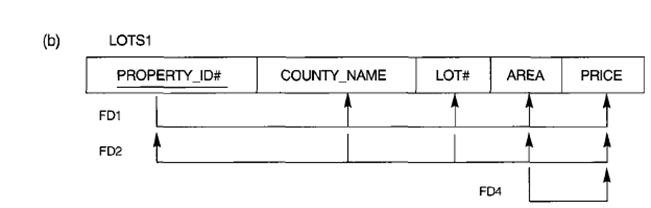
\includegraphics[scale=0.4]{img/normalization/norm13}
	\end{figure}
	
	If I want to add a new property in a lot with the same area of another one, I have to manually repeat the data about the PRICE for that AREA.
	
	It can be seen as a generalization of the previous 3NF where there must not be a transitive dependency also on a candidate key of the table
		
\end{frame}

\begin{frame}
	\frametitle{Normalization on candidate keys}
	\framesubtitle{Boyce-Codd normal form}
	
	\textbf{Definition:} A table is in Boyce-Codd normal form (BCNF) if for all non-trivial dependencies \fdep{X}{A} then X is a superkey of the table.
	
	\textbf{NOTE:} If a table is in BCNF then it is also in 3NF. Indeed to esnure the 3NF it is enough that only one between the BCNF condition and the other one (see the previous slide) is met.
	
	\begin{wrapfigure}{r}{0.5\textwidth}
		%\vspace{-20pt}
		\begin{center}
			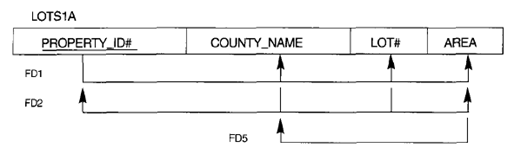
\includegraphics[scale=0.4]{img/normalization/norm13b}
		\end{center}
		%\vspace{-20pt}
		%\vspace{-10pt}
	\end{wrapfigure}
	
	\textbf{Example:} The table to the right is in 3NF but not in BCNF because COUNTY\textunderscore NAME depends on AREA, which is not a superkey.
	
\end{frame}

\SlideSection{Summary}

\begin{frame}
	\frametitle{Summary}
	\begin{itemize}
		\item Unnormalized tables might contain data redundancy and cause anomalies.
		\item Normal form are a way to solve these problems.
		\item There are normal form definitions for tables with just one key (the primary key and no candidate keys).
		\item There are normal form definitions for tables with candidate keys.
	\end{itemize}
\end{frame}


\end{document}

\begin{slide}{
\item ...
}\end{slide}

\begin{frame}[fragile]
\begin{lstlisting}
...
\end{lstlisting}
\end{frame}
